\documentclass[12pt]{article}
\usepackage[utf8]{inputenc}   % UTF-8 encoding
\usepackage{amsmath}          % For advanced math
\usepackage{amssymb}          % For symbols
\usepackage{geometry}         % To adjust margins
\usepackage{graphicx}         % For including images
\usepackage{hyperref}         % For clickable links
\usepackage{physics}          % Optional: easy physics notation
\usepackage{caption}          % Better captions
\usepackage{subcaption}
\usepackage{enumitem}         % Custom lists
\usepackage{titlesec}         % Customize section titles
\usepackage{float}

% Table
\usepackage[table]{xcolor}
\usepackage{colortbl}
\usepackage{array}
\usepackage{makecell}

% ---------- Page Setup ----------
\geometry{
	a4paper,
	left=25mm,
	right=25mm,
	top=25mm,
	bottom=25mm
}

% ---------- Title Info ----------
\title{
	\textbf{Principles of Data Communications and Networks Modeling (CS4865/6865)} \\[2mm]
	\textbf{}
	\text{Assignment \#1: Theoretical Channel Capacity}
}
\author{Abid Hasan Muin (3804634)}
\date{Due date: September 22, 2025}

% ---------- Section formatting ----------
\titleformat{\section}{\large\bfseries}{Question \thesection:}{1em}{}
\setcounter{section}{0}  % Start numbering from 1

\begin{document}
	
	\maketitle
	
	% Question 1
	
	\section{802.11b Wireless Channel}
	
	\subsection*{Given Data}
	\begin{itemize}[noitemsep]
		\item Transmitter power: $P_t = 0.1~\mathrm{W}$
		\item Channel bandwidth: $B = 22~\mathrm{MHz} = 22 \times 10^{6}~\mathrm{Hz}$
		\item Carrier frequency: $f = 2.4~\mathrm{GHz} = 2.4 \times 10^{9}~\mathrm{Hz}$
		\item Thermal noise temperature: $T = 400~\mathrm{K}$
		\item Boltzmann Constant: $k = 1.38 \times 10^{-23}~{J/K}$
		\item Speed of light: $c = 3 \times 10^{8}~{m/s}$
		\item Distance: $d = 10~\mathrm{m} \text{ to } 100~\mathrm{m}$
		\item Pi: $\pi = 3.14$
	\end{itemize}
	
	\subsection*{Calculations}
	
	The thermal noise is given by $N = kTB$, where $k$ is the Boltzmann constant, $T$ is the temperature in Kelvin, and $B$ is the bandwidth. Using given values $k = 1.38 \times 10^{-23}~\mathrm{J/K}$, $T = 400~\mathrm{K}$, and $B = 22 \times 10^6~\mathrm{Hz}$, the thermal noise is:
	
	\begin{equation*}
	N = (1.38 \times 10^{-23}) \times 400 \times (22 \times 10^6)
		\approx 1.21 \times 10^{-13}~\mathrm{W}	
	\end{equation*}
	
	\noindent
	The free space loss for isotropic antenna is given by $L = \frac{P_t}{P_r}$. From Friis transmission equation \cite{friis}, we can also denote $L = (\frac{4\pi fd}{c})^2$ , where $f$ is the carrier frequency, $d$ is the distance between transmitter and receiver, $c$ is the speed of light.\newline
	
	\noindent
	\textbf{For distance 10m:}
	
	\textit{Free space loss} is denoted by L,
	
	\begin{equation*}
		L = (\frac{4\pi fd}{c})^2 = [\frac{4 \times 3.14 \times (2.4 \times 10^{9}) \times 10}{3 \times 10^{8}}]^{2}
		\approx 1.01\times 10^{6}
	\end{equation*}

	\textit{Received signal strength} is denoted by S,
	\begin{equation*}
		S = P_r = \frac{P_t}{L} = \frac{0.1}{1.01 \times 10^{6}}
		\approx 9.9 \times 10^{-8}
	\end{equation*}

	\textit{Shannon capacity formula:}
	\begin{equation*}
		C = B \log_2 \left(1 + \frac{S}{N}\right) = (22 \times 10^6) \times \log_2 (1+\frac{9.9 \times 10^{-8}}{1.21 \times 10^{-13}})
		\approx 4.32 \times 10^{8}
	\end{equation*}
	
	\noindent
	\textbf{For distance 20m:}

	\textit{Free space loss} is denoted by L,

	\begin{equation*}
		L = (\frac{4\pi fd}{c})^2 = [\frac{4 \times 3.14 \times (2.4 \times 10^{9}) \times 20}{3 \times 10^{8}}]^{2}
		\approx 4.04 \times 10^{6}
	\end{equation*}
	
	\textit{Received signal strength} is denoted by S,
	\begin{equation*}
		S = P_r = \frac{P_t}{L} = \frac{0.1}{1.01 \times 10^{6}}
		\approx 2.48 \times 10^{-8}
	\end{equation*}
	
	\textit{Shannon capacity formula:}
	\begin{equation*}
		C = B \log_2 \left(1 + \frac{S}{N}\right) = (22 \times 10^6) \times \log_2 (1+\frac{2.48 \times 10^{-8}}{1.21 \times 10^{-13}})
		\approx 3.88 \times 10^{8}
	\end{equation*}

	\noindent
	\textbf{For distance 30m:}
	
	\textit{Free space loss} is denoted by L,
	
	\begin{equation*}
		L = (\frac{4\pi fd}{c})^2 = [\frac{4 \times 3.14 \times (2.4 \times 10^{9}) \times 30}{3 \times 10^{8}}]^{2}
		\approx 9.09 \times 10^{6}
	\end{equation*}
	
	\textit{Received signal strength} is denoted by S,
	\begin{equation*}
		S = P_r = \frac{P_t}{L} = \frac{0.1}{1.01 \times 10^{6}}
		\approx 1.10 \times 10^{-8}
	\end{equation*}
	
	\textit{Shannon capacity formula:}
	\begin{equation*}
		C = B \log_2 \left(1 + \frac{S}{N}\right) = (22 \times 10^6) \times \log_2 (1+\frac{1.10 \times 10^{-8}}{1.21 \times 10^{-13}})
		\approx 3.62 \times 10^{8}
	\end{equation*}

	\noindent
	\textbf{For distance 40m:}

	\textit{Free space loss} is denoted by L,
	
	\begin{equation*}
	L = (\frac{4\pi fd}{c})^2 = [\frac{4 \times 3.14 \times (2.4 \times 10^{9}) \times 40}{3 \times 10^{8}}]^{2}
	\approx 1.62 \times 10^{7}
	\end{equation*}
	
	\textit{Received signal strength} is denoted by S,
	\begin{equation*}
	S = P_r = \frac{P_t}{L} = \frac{0.1}{1.01 \times 10^{6}}
	\approx 6.19 \times 10^{-9}
	\end{equation*}
	
	\textit{Shannon capacity formula:}
	\begin{equation*}
	C = B \log_2 \left(1 + \frac{S}{N}\right) = (22 \times 10^6) \times \log_2 (1+\frac{6.19 \times 10^{-9}}{1.21 \times 10^{-13}})
	\approx 3.44 \times 10^{8}
	\end{equation*}
	
	\noindent
	\textbf{For distance 50m:}
	
	\textit{Free space loss} is denoted by L,
	
	\begin{equation*}
		L = (\frac{4\pi fd}{c})^2 = [\frac{4 \times 3.14 \times (2.4 \times 10^{9}) \times 50}{3 \times 10^{8}}]^{2}
		\approx 2.52 \times 10^{7}
	\end{equation*}
	
	\textit{Received signal strength} is denoted by S,
	\begin{equation*}
		S = P_r = \frac{P_t}{L} = \frac{0.1}{1.01 \times 10^{6}}
		\approx 3.96 \times 10^{-9}
	\end{equation*}
	
	\textit{Shannon capacity formula:}
	\begin{equation*}
		C = B \log_2 \left(1 + \frac{S}{N}\right) = (22 \times 10^6) \times \log_2 (1+\frac{3.96 \times 10^{-9}}{1.21 \times 10^{-13}})
		\approx 3.3 \times 10^{8}
	\end{equation*}
	
	\noindent
	\textbf{For distance 60m:}
	
	\textit{Free space loss} is denoted by L,
	
	\begin{equation*}
		L = (\frac{4\pi fd}{c})^2 = [\frac{4 \times 3.14 \times (2.4 \times 10^{9}) \times 60}{3 \times 10^{8}}]^{2}
		\approx 3.63 \times 10^{7}
	\end{equation*}
	
	\textit{Received signal strength} is denoted by S,
	\begin{equation*}
		S = P_r = \frac{P_t}{L} = \frac{0.1}{1.01 \times 10^{6}}
		\approx 2.75 \times 10^{-9}
	\end{equation*}
	
	\textit{Shannon capacity formula:}
	\begin{equation*}
		C = B \log_2 \left(1 + \frac{S}{N}\right) = (22 \times 10^6) \times \log_2 (1+\frac{2.75 \times 10^{-9}}{1.21 \times 10^{-13}})
		\approx 3.18 \times 10^{8}
	\end{equation*}
	
	\noindent
	\textbf{For distance 70m:}
	
	\textit{Free space loss} is denoted by L,
	
	\begin{equation*}
		L = (\frac{4\pi fd}{c})^2 = [\frac{4 \times 3.14 \times (2.4 \times 10^{9}) \times 70}{3 \times 10^{8}}]^{2}
		\approx 4.95 \times 10^{7}
	\end{equation*}
	
	\textit{Received signal strength} is denoted by S,
	\begin{equation*}
		S = P_r = \frac{P_t}{L} = \frac{0.1}{1.01 \times 10^{6}}
		\approx 2.02 \times 10^{-9}
	\end{equation*}
	
	\textit{Shannon capacity formula:}
	\begin{equation*}
		C = B \log_2 \left(1 + \frac{S}{N}\right) = (22 \times 10^6) \times \log_2 (1+\frac{2.02 \times 10^{-9}}{1.21 \times 10^{-13}})
		\approx 3.09 \times 10^{8}
	\end{equation*}
	
	\noindent
	\textbf{For distance 80m:}
	
	\textit{Free space loss} is denoted by L,
	
	\begin{equation*}
		L = (\frac{4\pi fd}{c})^2 = [\frac{4 \times 3.14 \times (2.4 \times 10^{9}) \times 80}{3 \times 10^{8}}]^{2}
		\approx 6.46 \times 10^{7}
	\end{equation*}
	
	\textit{Received signal strength} is denoted by S,
	\begin{equation*}
		S = P_r = \frac{P_t}{L} = \frac{0.1}{1.01 \times 10^{6}}
		\approx 1.55 \times 10^{-9}
	\end{equation*}
	
	\textit{Shannon capacity formula:}
	\begin{equation*}
		C = B \log_2 \left(1 + \frac{S}{N}\right) = (22 \times 10^6) \times \log_2 (1+\frac{1.55 \times 10^{-9}}{1.21 \times 10^{-13}})
		\approx 3.00 \times 10^{8}
	\end{equation*}
	
	\noindent
	\textbf{For distance 90m:}
	
	\textit{Free space loss} is denoted by L,
	
	\begin{equation*}
		L = (\frac{4\pi fd}{c})^2 = [\frac{4 \times 3.14 \times (2.4 \times 10^{9}) \times 90}{3 \times 10^{8}}]^{2}
		\approx 8.18 \times 10^{7}
	\end{equation*}
	
	\textit{Received signal strength} is denoted by S,
	\begin{equation*}
		S = P_r = \frac{P_t}{L} = \frac{0.1}{1.01 \times 10^{6}}
		\approx 1.22 \times 10^{-9}
	\end{equation*}
	
	\textit{Shannon capacity formula:}
	\begin{equation*}
		C = B \log_2 \left(1 + \frac{S}{N}\right) = (22 \times 10^6) \times \log_2 (1+\frac{1.22 \times 10^{-9}}{1.21 \times 10^{-13}})
		\approx 2.93 \times 10^{8}
	\end{equation*}
	
	\noindent
	\textbf{For distance 100m:}
	
	\textit{Free space loss} is denoted by L,
	
	\begin{equation*}
		L = (\frac{4\pi fd}{c})^2 = [\frac{4 \times 3.14 \times (2.4 \times 10^{9}) \times 100}{3 \times 10^{8}}]^{2}
		\approx 1.01 \times 10^{8}
	\end{equation*}
	
	\textit{Received signal strength} is denoted by S,
	\begin{equation*}
		S = P_r = \frac{P_t}{L} = \frac{0.1}{1.01 \times 10^{6}}
		\approx 9.9 \times 10^{-10}
	\end{equation*}
	
	\textit{Shannon capacity formula:}
	\begin{equation*}
		C = B \log_2 \left(1 + \frac{S}{N}\right) = (22 \times 10^6) \times \log_2 (1+\frac{9.9 \times 10^{-10}}{1.21 \times 10^{-13}})
		\approx 2.86 \times 10^{8}
	\end{equation*}
	
	\subsection{Data table of numerical values of distance and data rate}
	Below is the table with numerical values of distance and data rate which were calculated at 10m interval.
	
	\begin{table}[H]
		\centering
		\begin{tabular}{|c|c|c|}
			\hline
			% \rowcolor{gray!30}
			Serial No. & \makecell{Distance \\ (m)} & \makecell{Data rate \\ (Mbps)} \\ 
			\hline
			1 & 10 & 432 \\
			\hline
			2 & 20 & 388 \\
			\hline
			3 & 30 & 362 \\
			\hline
			4 & 40 & 344 \\
			\hline
			5 & 50 & 330 \\
			\hline
			6 & 60 & 318 \\
			\hline
			7 & 70 & 309 \\
			\hline
			8 & 80 & 300 \\
			\hline
			9 & 90 & 293 \\
			\hline
			10 & 100 & 286 \\
			\hline
 		\end{tabular}
		\caption{Numerical table of distance and data rate}
	\end{table}

	
	
	\subsection{Plot of Maximum Data Rate (Theoretical) vs Distance}
	After plotting the values that was calculated earlier, the following graph can be observed.
	\begin{figure}[H]
		\centering
		\label{fig:graph_1}
		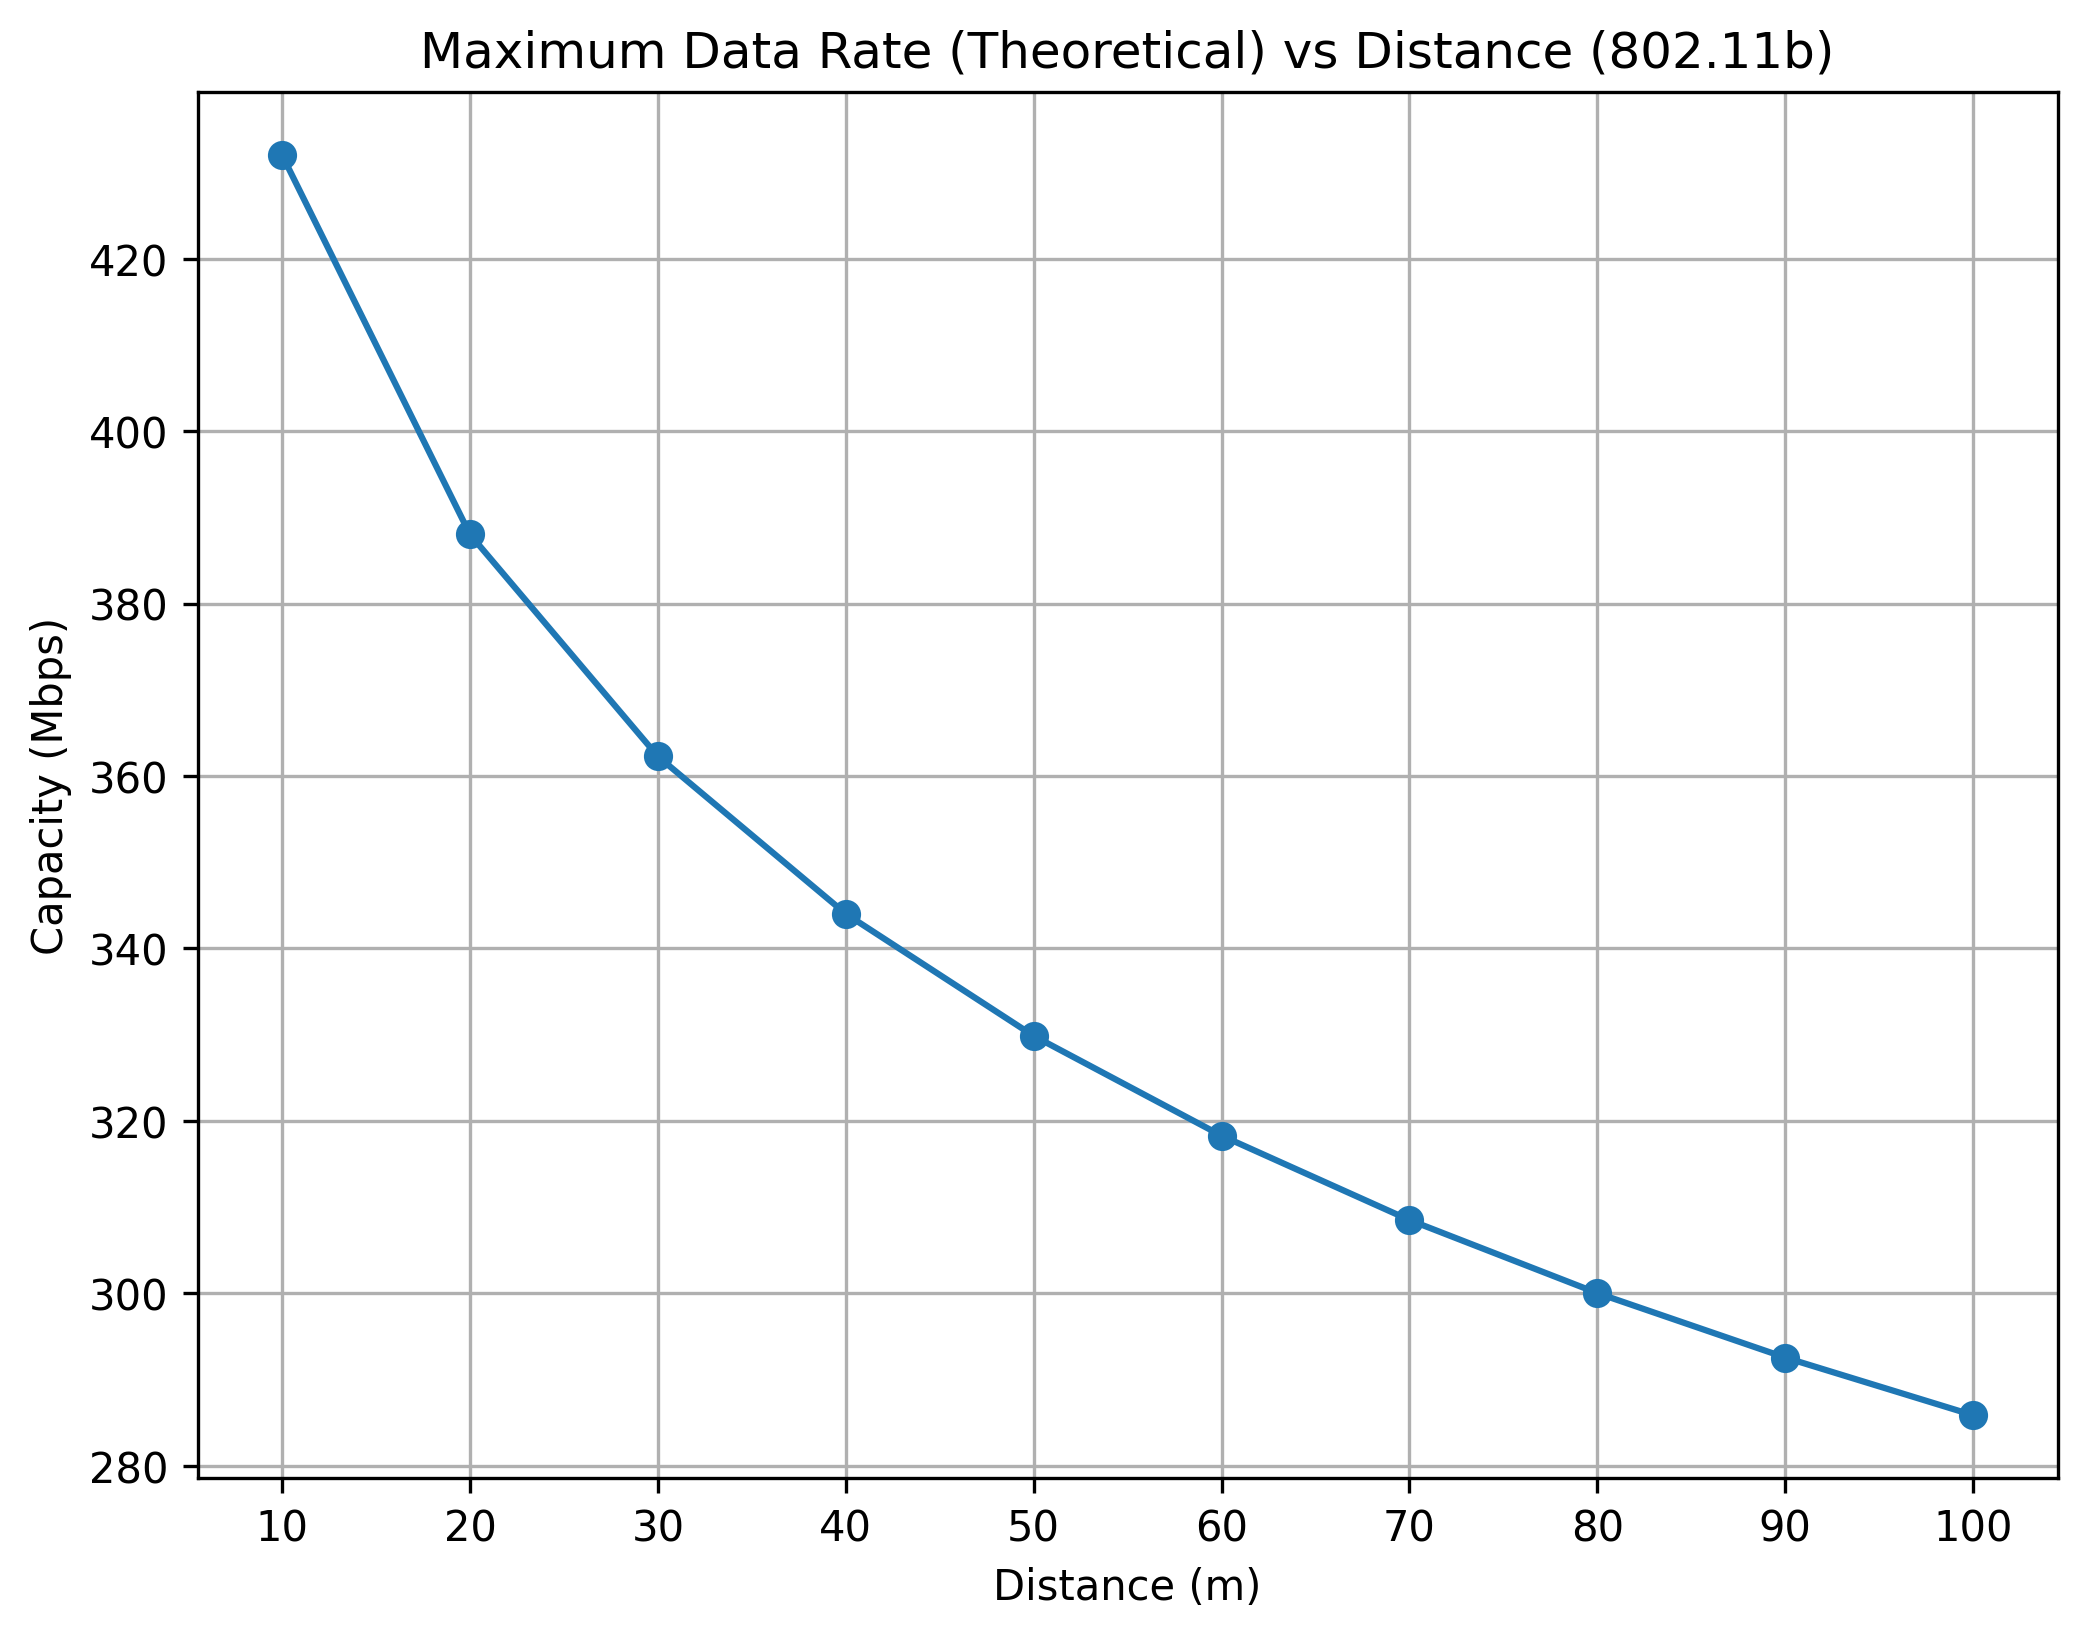
\includegraphics{graph}
		\caption{Maximum data rate (theoretical) for distances from 10m to 100 m}
	\end{figure}
	
	\hrule
	
	% Question 2
	
	\section{Comparison with the given research paper (Experimental Performance Evaluation of Wireless 802.11b Networks)}
	\subsection{Comparison of measured values}
	The measured values from the mentioned research paper and the calculated theoretical ones differ quite a lot. For reference, two graphs are shown below - 
	
	\begin{figure}[H]
		\centering
		\begin{subfigure}[b]{0.45\textwidth}
			\centering
			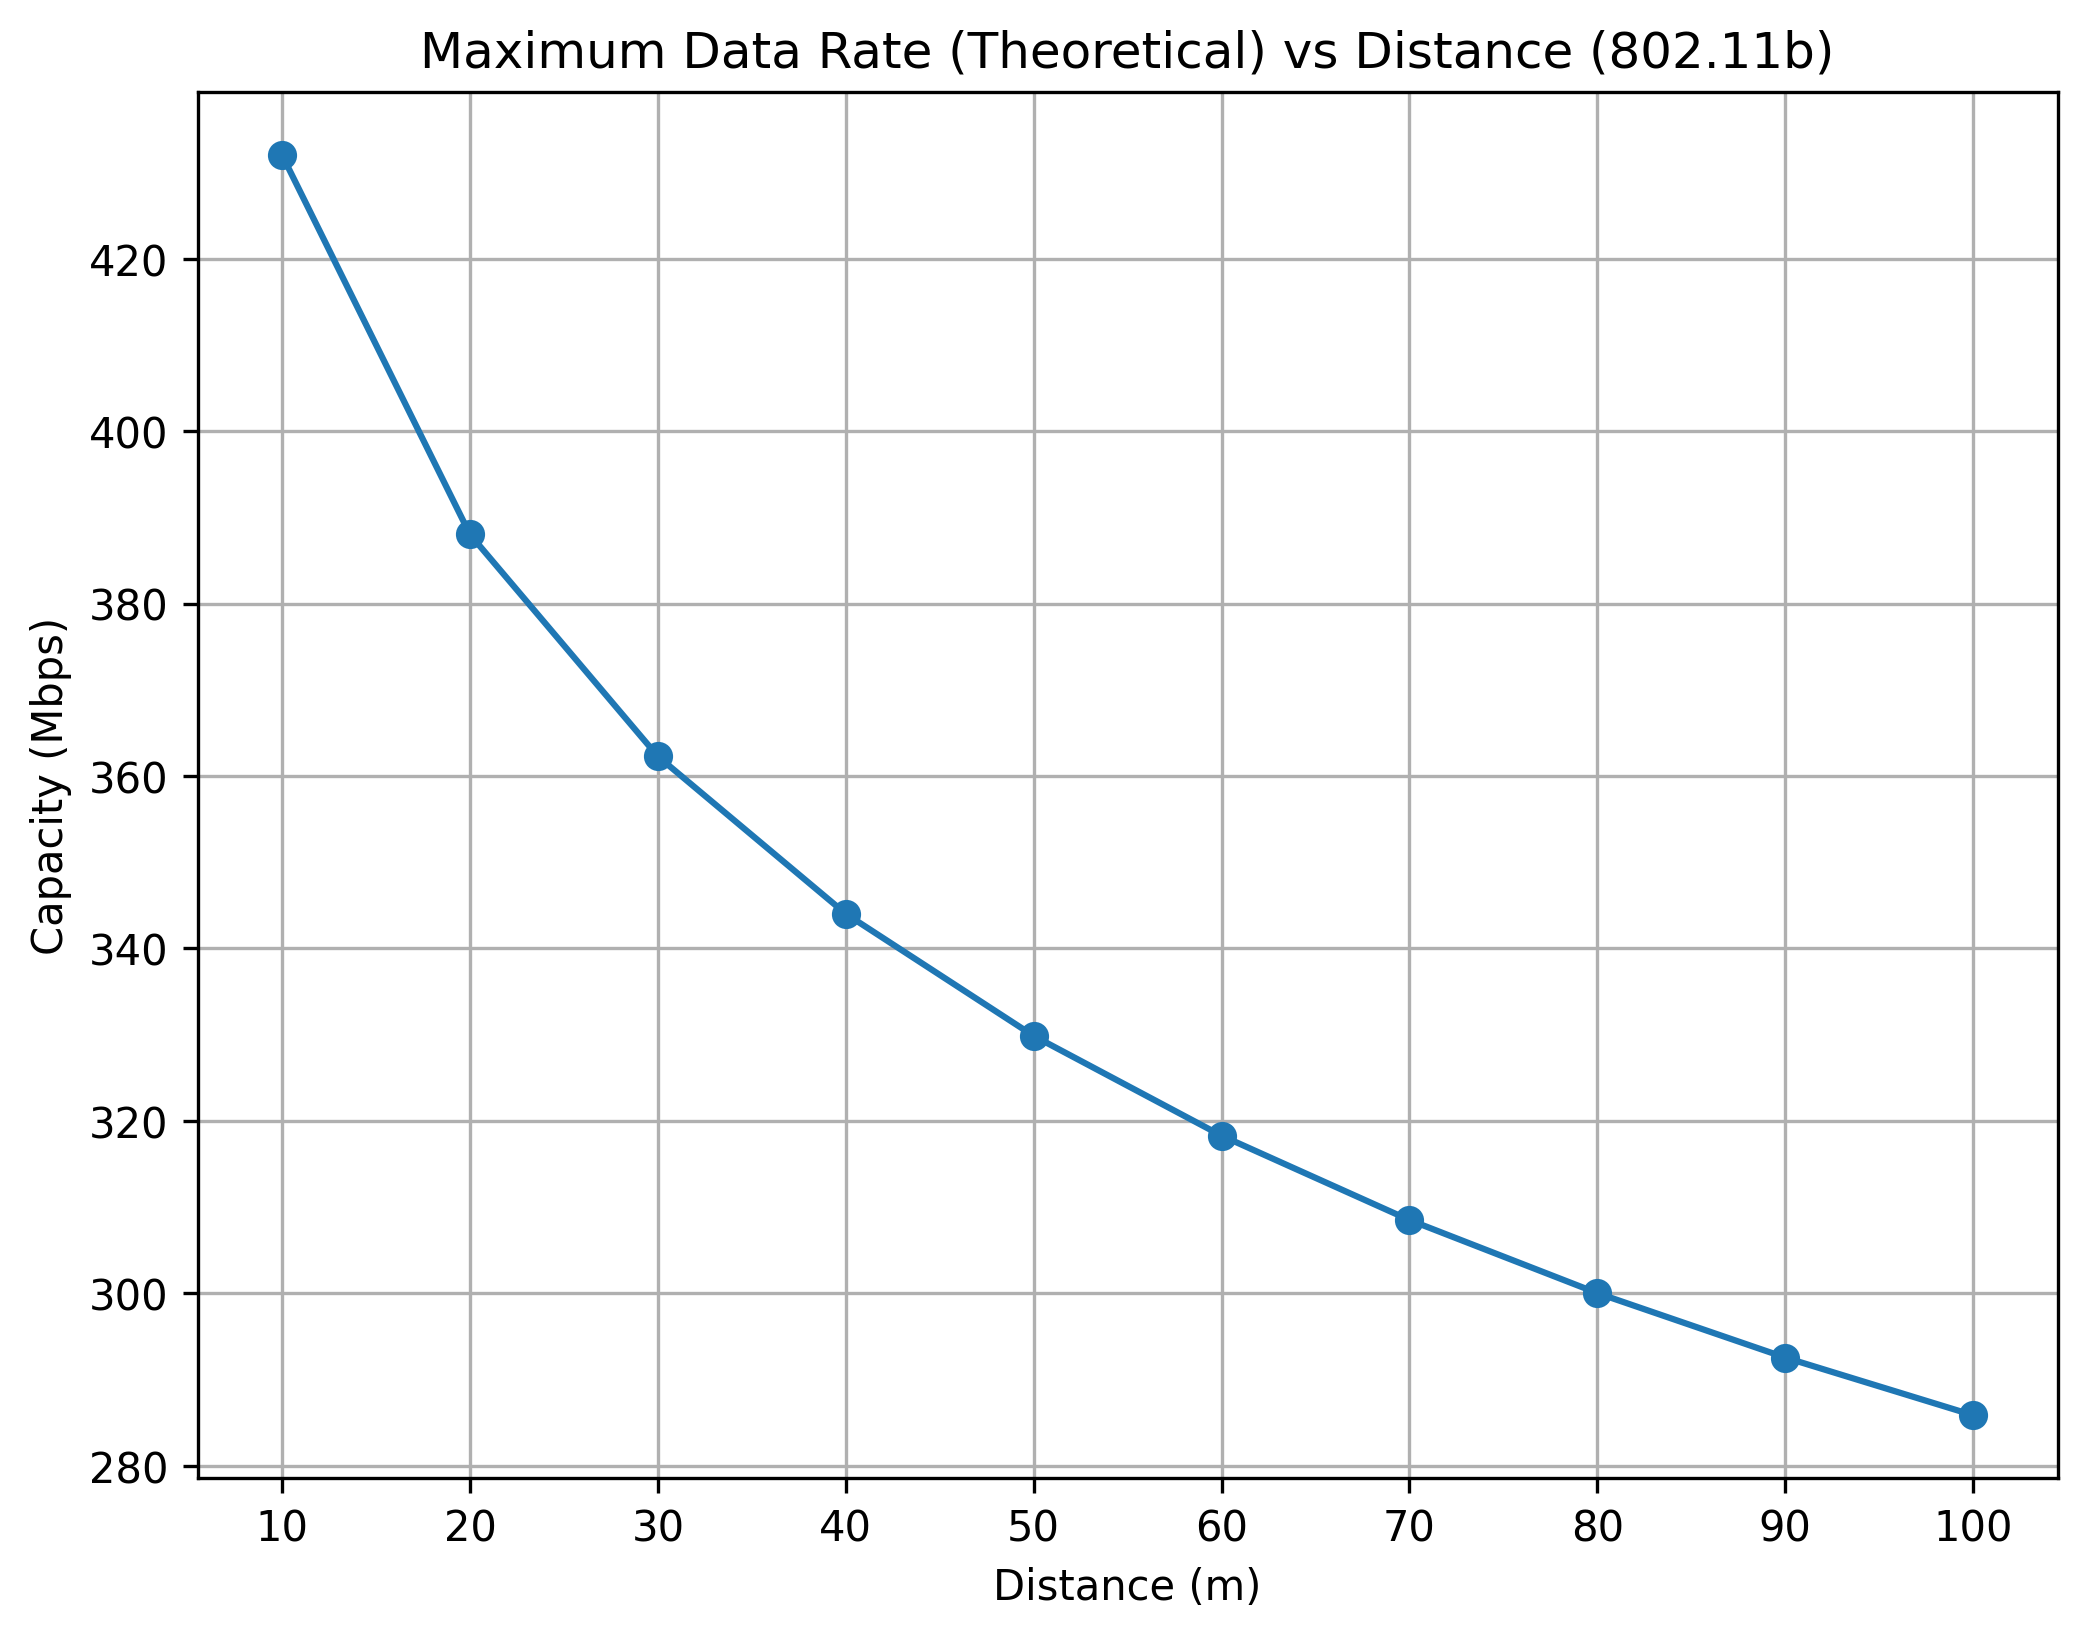
\includegraphics[width=\textwidth]{graph}
			\caption{Maximum data rate (theoretical)}
			\label{fig:graph_theoretical}
		\end{subfigure}
		\hfill
		\begin{subfigure}[b]{0.45\textwidth}
			\centering
			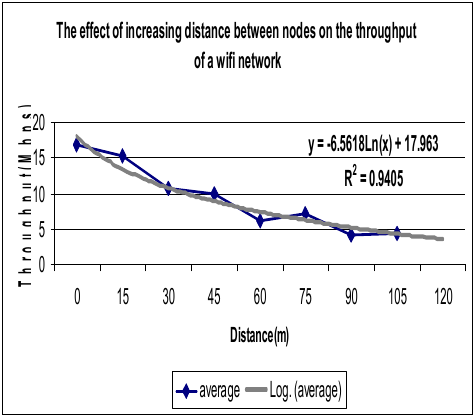
\includegraphics[width=\textwidth]{graph_measured}
			\caption{Measured data rate from paper}
			\label{fig:graph_measured}
		\end{subfigure}
		\caption{Value comparison of data rates between theoretical and practical}
		\label{fig:graph_paper}
	\end{figure}

	\subsection{Discussion of theoretical throughput and measured values in paper}
	Overall, the theoretical and measured values are not same. There are both similarities and dissimilarities in between theoretical throughput and measured values.
	
	\subsubsection{Similarities}
	
	\begin{itemize}[noitemsep]
		\item Both theoretical and measured data rate graphs show downward trend as distance increases. This is expected with wireless behavior where the signal strength decreases with increased distance.
	\end{itemize}
	
	\subsubsection{Dissimilarities}
	 
	\begin{itemize}[noitemsep]
		\item \textbf{Parameter Differences:} The parameters which were used to calculate the data rate of theoretical and measured one differs, such as - temperature, distance, network traffic etc. For theoretical, 10m interval is considered whereas in measured one it was 15m. Also, in case of theoretical data rate, interference was not considered as there was no real network traffic.
		
		\item \textbf{Experimental Devices:} In case of theoretical, a single device was considered. But in the measured one, there were three separate devices. In practical one, it introduced interference and performance was varied. Also a software \textit{Iperf} was used to measure the performance in case of the measured one. Devices used in the mentioned paper were not identical and thus their specifications were different which are absent in the theoretical one.
		
		\item \textbf{Protocol and Modulation Overheads:} In case of theoretical, the data rate calculation does not consider protocol overheads, such as modulation or CSMA/CA delays \cite{wiki}. But in measured one, these factors introduced additional latency and thus reduced the overall throughput which also lead to difference between theoretical and measured values.

	\end{itemize}
	
	\noindent
	The above points are my justification for why the theoretical calculated and measured values from the research paper differs.
	
	\hrule
	
	\section{Mars Rover Communication}
	
	\subsection*{Given Data}
	
	\begin{itemize}[noitemsep]
		\item Average Earth to Mars distance, $d = (\frac{100,000,000+400,000,000}{2})~\mathrm{km} = 2.5 \times 10^{11}~\mathrm{m}$
		\item Transmitter Power (Curiosity), $P_t = 15~\mathrm{W}$
		\item LGA gain (Curiosity), $G_t = 5~\mathrm{dBi}$
		
		\item Transmitter Power (DSN), $P_t = 20~\mathrm{kW}$
		\item Downlink carrier frequency (X-band), $f = 8.4~\mathrm{GHz}$
		\item DSN receive antenna gains (on-axis, X-band), $G_{r,34} = 68.3~\mathrm{dBi}$, $G_r,70 = 74.18~\mathrm{dBi}$
		
		\item Frequency (DTE - Downlink), $f_{dte} = 8.4~\mathrm{GHz}$
		\item Frequency (DFE - Uplink), $f_{dfe} = 7.2~\mathrm{GHz}$
		
		\item System noise temperature (receiver), $T_{sys,34} = 27~\mathrm{K}$, $T_{sys,70} = 17~\mathrm{K}$
		\item Bandwidth, $B = 500~\mathrm{kHz}$
		\item Boltzmann Constant, $k = 1.38 \times 10^{-23}~{J/K}$
		\item Speed of light, $c = 3 \times 10^{8}~{m/s}$
		
		\item Transmitter power, frequency, receiver noise, distance to Earth  
	\end{itemize}
	
	\subsection{Calculations}
	
	\subsubsection{Space Loss:}
	\textbf{For DTE (8.4 GHz):} The space loss is denoted by $L_s$,
	\begin{equation*}
		\lambda = \frac{c}{f} = \frac{3 \times 10^{8}}{8.4 \times 10^{9}} = 0.0357~\mathrm{m}
	\end{equation*}

	\begin{equation*}
		L_s = (\frac{\lambda}{4 \pi d})^{2} = (\frac{0.0357}{4 \pi \times 2.5 \times 10^{11}}) = 1.29 \times 10^{-28}
	\end{equation*}
	
	
	\textbf{For DFE (7.2 GHz):} The space loss is denoted by $L_s$,
	\begin{equation*}
		\lambda = \frac{c}{f} = \frac{3 \times 10^{8}}{7.2 \times 10^{9}} = 0.0417~\mathrm{m}
	\end{equation*}
	
	\begin{equation*}
		L_s = (\frac{\lambda}{4 \pi d})^{2} = (\frac{0.0417}{4 \pi \times 2.5 \times 10^{11}}) = 1.76 \times 10^{-28}
	\end{equation*}
	
	\subsubsection{Signal to Noise ratio:}
	\textbf{For DTE:} The signal to noise ratio is denoted by $SNR_{dte}$.
	
	\begin{equation*}
		SNR = \frac{P_t G_t G_r L_s L_o}{k T_{sys} B}
	\end{equation*}
	
	\noindent
	After converting gains to linear scale we get,
	$G_t = 10^{5/10} = 3.16$ and $G_r = 10^{68/10} = 6.31 \times 10^{6}$
	
	\begin{equation*}
		SNR_{dte} = \frac{15 \times 3.16 \times (6.31 \times 10^{6}) \times (1.29 \times 10^{-28}) \times 0.5}{(1.38 \times 10^{-23} \times 25 \times 500000)} = 1.12 \times 10^{-4}
	\end{equation*}
	
	\textbf{For DFE:} The signal to noise ratio is denoted by $SNR_{dfe}$.
	
	\begin{equation*}
		SNR = \frac{P_t G_t G_r L_s L_o}{k T_{sys} B}
	\end{equation*}
	
	\noindent
	After converting gains to linear scale we get,
	$G_t = 10^{5/10} = 3.16$ and $G_r = 10^{68/10} = 6.31 \times 10^{6}$
	
	\begin{equation*}
		SNR_{dfe} = \frac{20000 \times (6.31 \times 10^{6}) \times 3.16 \times (1.76 \times 10^{-28}) \times 0.5}{(1.38 \times 10^{-23} \times 25 \times 500000)} = 0.203
	\end{equation*}

	\subsection{Theoretical Maximum Data Rate Calculation}
	
	\subsubsection{DTE Data Rate:}
	
	\begin{equation*}
		C_{dte} = 50000 \times \log_2 (1+1.12 \times 10^{-4}) = 80.78 bps
	\end{equation*}
	
	\subsubsection{DFE Data Rate:}
	
	\begin{equation*}
		C_{dfe} = 50000 \times \log_2 (1+0.203) = 13331.83 bps
	\end{equation*}
	
	\section*{References}
	\begin{thebibliography}{9}
		\bibitem{wiki} WiFi standard 802.11b: \url{https://en.wikipedia.org/wiki/IEEE_802.11b-1999}
		\bibitem{friis} Friis transmission equation: \url{https://en.wikipedia.org/wiki/Friis_transmission_equation}
		\bibitem{paper} A.B. Fadhah et al., \textit{Experimental performance evaluation of Wireless 802.11b networks}, 2008 ICADIWT
		\bibitem{nasa} NASA, Communicating with Curiosity: \url{https://science.nasa.gov/resource/communicating-with-curiosity-2/}
		\bibitem{mars} S. Gordon, Communications with Mars Curiosity: \url{https://sandilands.info/sgordon/communications-with-mars-curiosity}
	\end{thebibliography}
	
\end{document}
